% CREATED BY DAVID FRISK, 2016

% IMPORT SETTINGS
\documentclass[12pt,a4paper,twoside,openright]{report}
% CREATED BY DAVID FRISK, 2016

% NOTE(Bjorn): Added packages.
\usepackage{verbatim}                   % For block comments
\usepackage{verbatimbox}
\usepackage{cite}
% BASIC SETTINGS
\usepackage{moreverb}                   % List settings
\usepackage{textcomp}                   % Fonts, symbols etc.
\usepackage{lmodern}                    % Latin modern font
\usepackage{helvet}                     % Enables font switching
\usepackage[T1]{fontenc}                % Output settings
\usepackage[english]{babel}             % Language settings
\usepackage[utf8]{inputenc}             % Input settings
\usepackage{amsmath}                    % Mathematical expressions
\usepackage{amssymb}                    % Mathematical symbols
\usepackage{graphicx}                   % Figures
\usepackage{wrapfig}					% Figures with text wrapping
\usepackage{subfig}                     % Enables subfigures
\numberwithin{equation}{chapter}        % Numbering order for equations
\numberwithin{figure}{chapter}          % Numbering order for figures
\numberwithin{table}{chapter}           % Numbering order for tables
\usepackage{listings}                   % Enables source code listings
\usepackage{chemfig}                    % Chemical structures
\usepackage[top=3cm, bottom=3cm,
            inner=3cm, outer=3cm]{geometry}     % Page margin lengths
\usepackage{eso-pic}                    % Create cover page background
\newcommand{\backgroundpic}[3]{
        \put(#1,#2){
        \parbox[b][\paperheight]{\paperwidth}{
        \centering
        \includegraphics[width=\paperwidth,height=\paperheight,
                         keepaspectratio]{#3}}}}
\usepackage{float}                      % Enables object position enforcement using[H]
\usepackage{parskip}                    % Enables vertical spaces correctly 



% Caption settings (aligned left with bold name)
\usepackage[labelfont=bf, textfont=normal,
                        justification=justified,
                        singlelinecheck=false]{caption}                 

                        
% Activate clickable links in table of contents         
\usepackage{hyperref}                                                           
\hypersetup{colorlinks, citecolor=black,
            filecolor=black, linkcolor=black,
            urlcolor=black}


% Define the number of section levels to be included in the t.o.c. 
% and numbered (3 is default)   
\setcounter{tocdepth}{5}                                                        
\setcounter{secnumdepth}{3}     


% Chapter title settings
\usepackage{titlesec}           
\titleformat{\chapter}[display]
  {\Huge\bfseries\filcenter}
  {{\fontsize{50pt}{1em}\vspace{-4.2ex}\selectfont \textnormal{\thechapter}}}{1ex}{}[]


% Header and footer settings (Select TWOSIDE or ONESIDE layout below)
\usepackage{fancyhdr}                                                           
\pagestyle{fancy}  
\renewcommand{\chaptermark}[1]{\markboth{\thechapter.\space#1}{}} 
\newcommand{\clash}{C$\lambda$aSH }


% Select one-sided (1) or two-sided (2) page numbering
\def\layout{2}  % Choose 1 for one-sided or 2 for two-sided layout
% Conditional expression based on the layout choice
\ifnum\layout=2 % Two-sided
    \fancyhf{}                                                                  
        \fancyhead[LE,RO]{\nouppercase{ \leftmark}}
        \fancyfoot[LE,RO]{\thepage}
        \fancypagestyle{plain}{                 % Redefine the plain page style
        \fancyhf{}
        \renewcommand{\headrulewidth}{0pt}              
        \fancyfoot[LE,RO]{\thepage}}    
\else                   % One-sided     
        \fancyhf{}                                      
        \fancyhead[C]{\nouppercase{ \leftmark}}
        \fancyfoot[C]{\thepage}
\fi


% Enable To-do notes
\usepackage[textsize=tiny]{todonotes} % Include the option "disable" to hide all notes
\setlength{\marginparwidth}{2.5cm} 


% Supress warning from Texmaker about headheight
\setlength{\headheight}{15pt}           


\begin{document} 

% COVER PAGE, TITLE PAGE AND IMPRINT PAGE
% Roman numbering (starting with i (one)) until first main chapter
\pagenumbering{roman}

%%%%%%%%%%%%%%%%%%%%%%%%%%%%%%%%%%%%%%%%%%%%%%%%%%%%%%%%%%
% NOTE(Bjorn):Global Variables for the frontmatter section.
%%%%%%%%%%%%%%%%%%%%%%%%%%%%%%%%%%%%%%%%%%%%%%%%%%%%%%%%%%
% An Informative Headline describing\\ the Content of the Report
\newcommand{\varHeadline}{First Attempt at a GPU \\ Tailored for Ray Marching}
% A Subtitle that can be Very Much Longer if Necessary
\newcommand{\varSubtitle}{A rudimentary GPU written in Clash(Haskell) compiled to VHDL}
% Department of Some Subject or Technology
\newcommand{\varDepartment}{Department of Computer Science and Engineering}
% Division of Division name
\newcommand{\varDivision}{Undergrad}
% Name of research group (if applicable)
\newcommand{\varResearchGroupName}{DATX-02-17-12}
% NAME FAMILYNAME
\newcommand{\varNames}{André Perzon, Björn Strömberg, Chi Thong Luong,  \\
Elias Forsberg, Jesper Åberg, Jon Johnsson}

% CREATED BY DAVID FRISK, 2016

% COVER PAGE
\begin{titlepage}
\newgeometry{top=3cm, bottom=3cm,
			left=2.25 cm, right=2.25cm}	% Temporarily change margins		
			
% Cover page background 
\AddToShipoutPicture*{\backgroundpic{-4}{56.7}{figure/auxiliary/frontpage_eng.pdf}}
\addtolength{\voffset}{2cm}

% Cover picture (replace with your own or delete)		
\begin{figure}[H]
\centering
\vspace{2cm}	% Adjust vertical spacing here
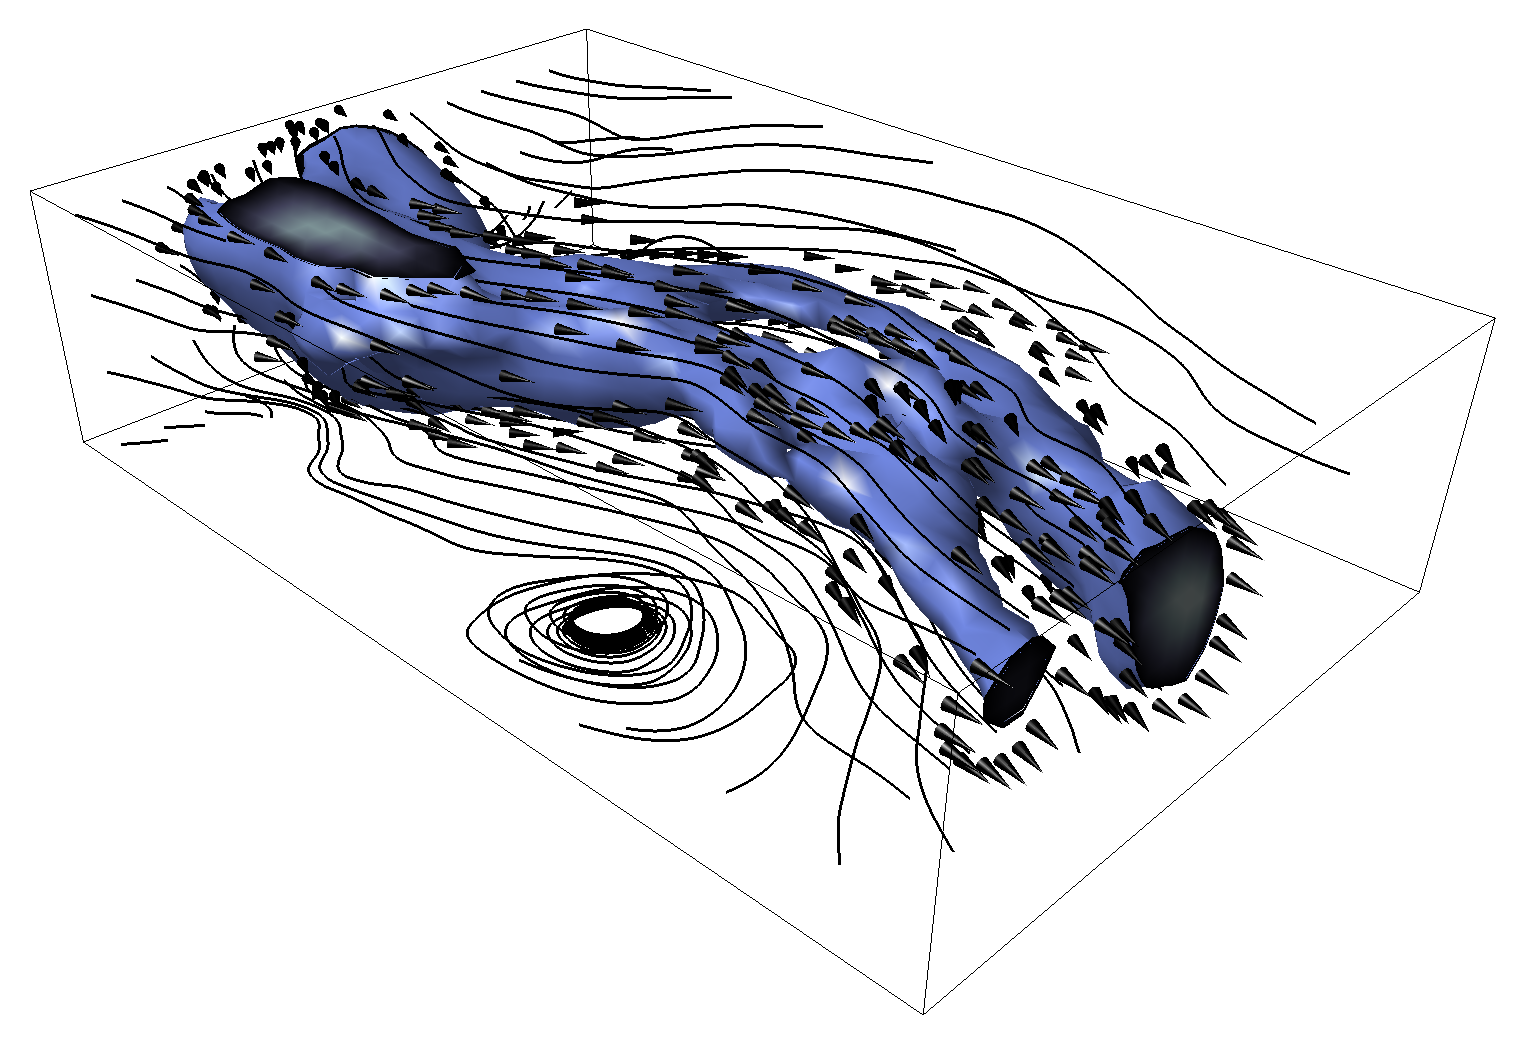
\includegraphics[width=0.9\linewidth]{figure/Wind.png}
\end{figure}

% Cover text
\mbox{}
\vfill
\renewcommand{\familydefault}{\sfdefault} \normalfont % Set cover page font
\textbf{{\Huge 	\varHeadline}} 	\\[0.5cm]
{\Large \varSubtitle}\\[0.5cm] Bachelor's thesis in Computer Science \setlength{\parskip}{1cm}

{\Large \varNames} \setlength{\parskip}{2.9cm}

\varDepartment \\
\textsc{Chalmers University of Technology} \\
Gothenburg, Sweden 2016

\renewcommand{\familydefault}{\rmdefault} \normalfont % Reset standard font
\end{titlepage}


% BACK OF COVER PAGE (BLANK PAGE)
\newpage
\restoregeometry
\thispagestyle{empty}
\mbox{}


% TITLE PAGE
\newpage
\thispagestyle{empty}
\begin{center}
	\textsc{\large Master's thesis 2016:NN}\\[4cm]		% Report number given by department 
	\textbf{\Large \varHeadline} \\[1cm]
	{\large \varSubtitle}\\[1cm]
	{\large \varNames}
	
	\vfill	
	% Logotype on titlepage	
	\begin{figure}[H]
	\centering
	% Remove the following line to remove the titlepage logotype
	
\includegraphics[width=0.2\pdfpagewidth]{figure/auxiliary/logo_eng.pdf} \\	
	\end{figure}	\vspace{5mm}	
	
	\varDepartment \\
	\emph{\varDivision}\\
	\varResearchGroupName\\
	\textsc{Chalmers University of Technology} \\
	Gothenburg, Sweden 2016 \\
\end{center}


% IMPRINT PAGE (BACK OF TITLE PAGE)
\newpage
\thispagestyle{plain}
\vspace*{4.5cm}
\varHeadline \\
\varSubtitle \\
\varNames \setlength{\parskip}{1cm}

\copyright ~ \varNames, 2016. \setlength{\parskip}{1cm}

Supervisor: Name, Company or Department\\
Examiner: Name, Department \setlength{\parskip}{1cm}

Master's Thesis 2016:NN\\	% Report number given by department 
\varDepartment \\
\varDivision \\
\varResearchGroupName\\
Chalmers University of Technology\\
SE-412 96 Gothenburg\\
Telephone +46 31 772 1000 \setlength{\parskip}{0.5cm}

\vfill
% Caption for cover page figure if used, possibly with reference to further information in the report
Cover: Wind visualization constructed in Matlab showing a surface of constant wind speed along with streamlines of the flow. \setlength{\parskip}{0.5cm}

Typeset in \LaTeX \\
Printed by [Name of printing company]\\
Gothenburg, Sweden 2016



% ABSTRACT
\newpage
\thispagestyle{plain}			% Supress header 
\setlength{\parskip}{0pt plus 1.0pt}

\section*{Abstract}
	
	Real-time rendering speed has always been a significant factor for 3D
	graphic cards. However, 3D graphic cards today are optimized and built for
	the polygon-based rendering. Therefore, Sphere Tracing rendering is slower
	in this hardware.  The aim of this thesis is to implement and design a
	basic GPU (Graphic proccesing unit) that could execute Sphere tracing.
	Subsequent to this, some optimizations were implemented in order to further
	assess the potential performance of the Sphere Tracing algorithm.
	
	This thesis documents the result of us examining the Sphere Tracing
	algorithm and designing a Graphics Processing Unit (GPU) to run it, using
	\clash, a functional hardware description language. In addition, possible
	future work are discussed.

	% KEYWORDS (MAXIMUM 10 WORDS)
	\vfill
	Keywords: sphere tracing, ray marching, ray tracing, GPU, real-time rendering.

\newpage
\thispagestyle{plain}

\section*{Sammanfattning}
	
	Denna uppsats dokumenterar resultaten kring en grafikenhet (GPU) som vi
	designat med avseende att köra en specifik rendreringsalgoritm kallad Sphere
	Tracing, en typ av Ray Tracing. GPUn är skriven i det funktionella
	hårdvarubeskrivande programmeringsspråket (FHDL) \clash.
	
	Hastigheten på realtidsrenderingen hos 3D grafikkort har alltid varit en
	viktig säljpunkt. Dock, när det kommer till Sphere Tracing rendrering jämfört
	med polygonbaserade rendreringsmetoder så har den förstnämda historiskt sett
	varit långsammare. Detta har lett till att man vidareutvecklat hårdvaran
	specifikt för att accelerera polygonrendrering vilket leder till frågan hur
	pass snabbt Sphere Tracing kan köras om liknande hårdvara skräddarsys för
	just den algoritmen. Avsikten med denna rapporten är att ge en idé om vilka
	prestandaökningar som finns att uppnå med ett alternativt realtidsrenderande
	3D grafikkort.
	
	% KEYWORDS (MAXIMUM 10 WORDS)
	\vfill
	Nyckelord: bollkoll, sphere tracing, ray marching, ray tracing, realtidsrendering.


\newpage
\thispagestyle{empty}
\mbox{}


% TABLE OF CONTENTS
\newpage
\tableofcontents

% TODO(Bjorn): Do we really want this?
\begin{comment}
% OTHER FRONTMATTER
% List of figures (add to table of contents)
\cleardoublepage
\addcontentsline{toc}{chapter}{\listfigurename} 
\listoffigures
% List of tables (add to table of contents)
\cleardoublepage
\addcontentsline{toc}{chapter}{\listtablename}  
\listoftables
\end{comment}

% START OF MAIN DOCUMENT
%\cleardoublepage
\newpage
\setcounter{page}{1}
\pagenumbering{arabic}			% Arabic numbering starting from 1 (one)
\setlength{\parskip}{0pt plus 1pt}

% INTRODUCTION
% CREATED BY DAVID FRISK, 2016
\chapter{Introduction} 

The algorithm in question that we designed a custom GPU for is called sphere
tracing.\cite{Hart1996} So called since it uses spheres to incrementally
advance a ray in 3D space. The method of advancing rays incrementally is called
ray marching and is a particular subset of ray tracing.\cite{Whitted1980} Ray
tracing, then, is a way of wholly or partially rendering the world through
rays, cast from the eye of the observer into the scene.  Sphere tracing has
been around since at least as early as the late eighties and ray tracing as
early as the sixties.\cite{Hart1989,Appel1968} Since ray tracing traditionally
has been a more computation-intensive method compared to
scanlining\cite{Wylie1967} and as such it has generally seen more use in movie
production rather than in real-time applications.\cite{ref_needed?} 

%TODO(bjorn): Nån som är bätre än mig på detta får gärna skriva om denna delen
%             nedanför. låter inte proffsigt alls.

The advent of the programmable shader brought back the discussion of real time
ray marching to the forefront. which is where we caught on to it.
\cite{JamieWong2016} It still favours poorly compared to other techniques which
natrually begged the question if it would be able to compete in real time if
only the hardware for it was there.

\section{Sphere tracing} 

\begin{minipage}{0.6\textwidth} 

	At the base of the algorithm are the signed distance functions.
	$$\text{SDF}:\mathbb{R}^{3}\mapsto\mathbb{R}$$ The "distance" is the distance
	between a point and the closest point on the implicit surface
	$\text{SDF}^{-1}(0)$. The "signed" part refers to the distance being negated
	when measured inside of the surface.  If we define a ray $$r(s) = \vec{d}
	\cdot s + \vec{o}$$ where $\vec{d}$ is the normalized direction of the ray
	and $\vec{o}$ the origin, then $$\text{SDF}\circ r(s) = 0$$ means that the
	ray intersects a surface at exactly the distance $s$ from its origin.

\end{minipage} 

\hfill
\begin{minipage}{0.3\textwidth}
	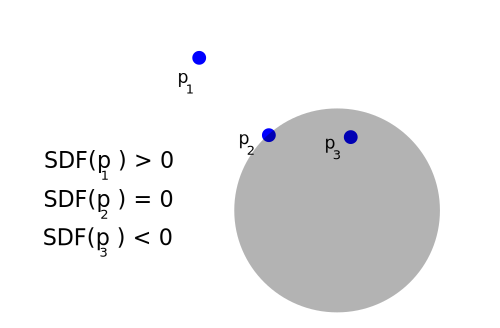
\includegraphics[width=\linewidth]{figure/SDF} 
\end{minipage}

\bigskip

Finding the surface can be done by iterating point by point from the origin
along the ray like below. $$p_{i+1} = p_i + \vec{d}\cdot \text{SDF}(p_i)$$ This
is repeated until $\text{SDF}(p_i) \leq \varepsilon$ for a given precision
limit $\varepsilon$. $\text{SDF}(p_i)$ is the furthest we can march the ray
while still be sure we don't overshoot any potential surfaces.  The direction
of the closest surface point is never known thus $\text{SDF}(p_i)$ can be
interpreted as a sphere bound, giving the algorithm its namesake. This ray
marching is then performed for each pixel of the screen reversely simulating
the light rays from a scene entering the lens of the onlooker.
	
	\subsection{Reflections and refractions}

	Once a point on a surface for a given pixel has been located new multiple
	rays can then be further marched to determine reflections, towards the
	scene's sources of light determening light and shadows, or through the object
	with an angle, simulating refractions. A lot of these depend on the surface
	normal which can be calculated by normalizing the aproximate gradient of
	$\text{SDF}(p)$. 

	\subsection{Textures}

	Texturizing could at least be done in two ways. The straightforward way would
	be to use the surface point coupled with an id-signature of the figure. After
	translating and re-scaling the point to the origin, it could then be directly
	looked up in a 1:1 3D texture as per its id. A more indirect but space-saving
	alternative could be to replace the last step with a sphere trace from the
	translated point along its surface normal\footnotemark out towards a simple
	wrapping geometry. The resulting surface coordinate could then along with the
	whole surface be transformed into a 2D flat plane mapping to a corresponding
	2D texture. The texture and enclosing geometry again being variable according
	to the id of the figure.

	\footnotetext{Or along the normal of the point.}

\section{Hardware implementation}


% THEORY
% CREATED BY DAVID FRISK, 2016
\chapter{Sphere Tracing} \label{spheretracing}

	% TODO(bjorn):
	% fixa bild r krockar

	The graphics rendering algorithm in question that we designed a custom GPU
	for is called Sphere Tracing\cite{Hart1996}. The name comes from the
	technique where it uses spheres to incrementally advance a ray in 3D space.
	The method of advancing rays incrementally is called Ray Marching and is a
	particular subset of ray tracing\cite{Whitted1980}. Ray Tracing, then, is a
	way of wholly or partially render the world through rays, cast from the eye
	of the observer into the scene. Sphere Tracing has been around since at least
	as early as the late eighties\cite{Hart1989} and Ray Tracing as early as the
	sixties\cite{Appel1968}. Ray Tracing has traditionally been a more
	computationally intensive method compared to polygon
	rendering\cite{Wylie1967} and thus it has generally seen more use in movie

	production rather than in real-time applications.\cite{ref_needed?} 

	The advent of per pixel programmable hardware in graphics cards made it 
	possible to implement real time graphics rendering based on ray	marching, 
	albeit only using relatively simple geometry. This raises the question of 
	whether this rendering method could be competitive for real time graphics 
	if hardware that was specifically designed for it was available.

	In this chapter we walk through the Sphere Tracing algorithm in detail with
	both definitions and examples. The explanation is based on the the very
	succint explanation in \cite{Korndorfer2014} where they also expand upon the
	original algorithm. For a more in-depth description we refer to Harts
	``\emph{Sphere tracing: a geometric method for the antialiased ray tracing
	of implicit surfaces}``\cite{Hart1996} as the de-facto explanation.


	\section{Sphere Tracing} 

		\begin{wrapfigure}{r}{0.48\textwidth}
			\begin{flushright}
				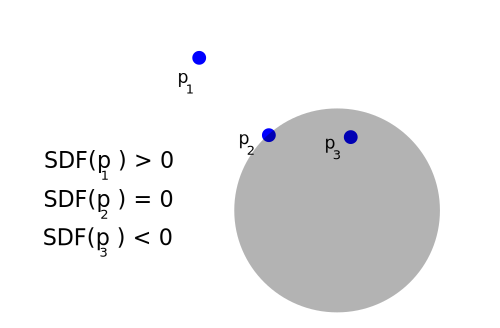
\includegraphics[width=0.9\linewidth]{figure/SDF} 
			\end{flushright}
			\caption{ Signed Distance Function of a sphere, sampled at three points}
			\vspace{40pt}
		\end{wrapfigure}

		The sphere tracing algorithm is based on the concept of Signed Distance
		Functions (SDF).  $$\text{SDF}:\mathbb{R}^{3}\mapsto\mathbb{R}$$ The
		``distance`` is the distance between a point and the closest point on the
		implicit surface $\text{SDF}^{-1}(0)$. The ``signed`` part refers to the
		distance being negated when measured on the other side of the surface. 

		A common example would be the SDF of a sphere centered at the origin with a
		radius of one. $$\text{SDF}(\vec{v}) = |\vec{v}| - 1$$ We can here see that
		a point $\vec{v}$ exactly on the surface would evaluate to $1 - 1 = 0$
		where any point outside of the sphere being positive and any point inside
		the sphere being negative. In this case the absolute of the result would
		also describe the smallest distance to the surface but this is not a hard
		constriction for the algorithm to work.

		\vspace{40pt}
		\begin{wrapfigure}{r}{0.48\textwidth}
			\begin{flushright}
				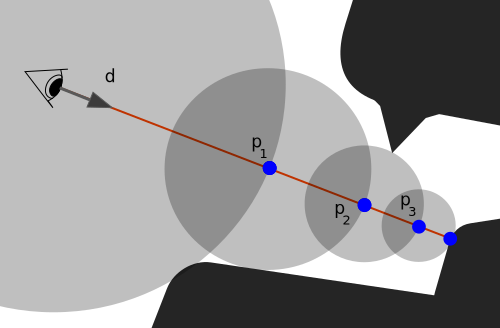
\includegraphics[width=0.9\linewidth]{figure/SDF2} 
			\end{flushright}
			\caption{A single ray marching according to Sphere Tracing}
			\vspace{40pt}
		\end{wrapfigure}

		If we define a ray $$r(s) = \vec{d} \cdot s + \vec{o}$$
		where $\vec{d}$ is the direction of the ray and $\vec{o}$ the origin, then
		$$\text{SDF}\circ r(s) = 0$$ means that the ray intersects a surface at
		exactly the distance $s$ from its origin. \emph{Sampling every SDF in a
		given scene and returning the smallest value yields a function known as a
		distance field.}

		\bigskip \noindent Finding the surface can be done by iterating point by
		point from the origin along the ray like below: $$p_{i+1} = p_i +
		\vec{d}\cdot \text{SDF}(p_i)$$ This is repeated until $\text{SDF}(p_i) \leq
		\varepsilon$ for a given precision limit $\varepsilon$. $\text{SDF}(p_i)$
		is the furthest possible march distance the ray can march while still being
		sure not too overshoot any potential surfaces. The direction of the closest
		surface point is never known, thus $\text{SDF}(p_i)$ can be interpreted as
		a spherical bound, giving the algorithm it's name. This Ray Marching is
		then performed for each pixel of the screen, reversely simulating the light
		rays entering the lens of an eye or camera.

			\subsection{Reflections, refractions and shading}

				Once a point on a surface for a given pixel has been located
				reflections, light, shadows and refractions needs to be calculated. A
				lot of these depend on the surface normal which can be approximated by
				the partial derivatives around the surface point for some small delta
				$\delta$, i.e taking the gradient and then normalizing it.

				$$\vec{g} = \vec{x}\cdot\frac{\text{SDF}(x+\delta, y, z)}{\delta} +
				\vec{y}\cdot\frac{\text{SDF}(x, y+\delta, z)}{\delta} +
				\vec{z}\cdot\frac{\text{SDF}(x, y, z+\delta)}{\delta} $$

				$$\vec{n} = \frac{\vec{g}}{|\vec{g}|} $$

				A simple way to lightset the scene could for an example be to use Phong
				Lightning\cite{Phong}. But from here on out any number of algorithms
				can be used in combination to determine the final color. Shadows can be
				determined by further Sphere Tracing out towards the sources of light
				to check for obstructions. Same for reflections and refractions where
				further marching in proportionate angles to the angle of incidence can
				determine what objects add to surface.


% METHODS
% CREATED BY DAVID FRISK, 2016
\chapter{Methods}


% RESULTS
\chapter{Results}

	In this chapter the results of GPU design choices and algorithmic
	optimizations and their effects are reviewed.

	\section{Software Shader Performance}

		The shader performed as expected, a conventional graphics card is
		capable of rendering scenes with low scene complexity in real-time
		using sphere tracing.

		Scenes can easily be made to look a lot more complex than they
		are, for example, by using mod fields, when the modulo
		operation is used on an object it creates a field with multiple copies
		of the original object next to each other, or fractals. The hardware
		(Geforce GTX 1060M) that the shader was tested on was able to render 20
		reflective spheres in real time in fullHD using our performance
		enhancing algorithm.
 
	\section{GPU}
	
		The GPU has been tested by simulating it and running a program on the simulation 
		that renders a sphere using Sphere Tracing. It spawns threads
		progressively to fill the screen data buffer with pixels. The execution
		of our test programs ran exactly as intended, with any number of
		simulated cores. The design has also been put through a synthesizing
		tool for FPGAs, which creates a net list of the components and
		connections that constitute the GPU. This also works as intended
		without any unexpected problems, but the actual operation of the GPU on
		an FPGA has not yet been verified.
	
	\section{Square roots}
		
		The accuracy of the different square root approximation and calculation
		methods are shown in figures \ref{sres1}, \ref{sres2}, \ref{sres3},
		\ref{sres4}, \ref{sres5}, and \ref{sres6}. The shifting nth root
		algorithm is used as a reference in all figures because it is always
		bit-accurate for integer square roots.

		\begin{figure}[H]
			\centering
			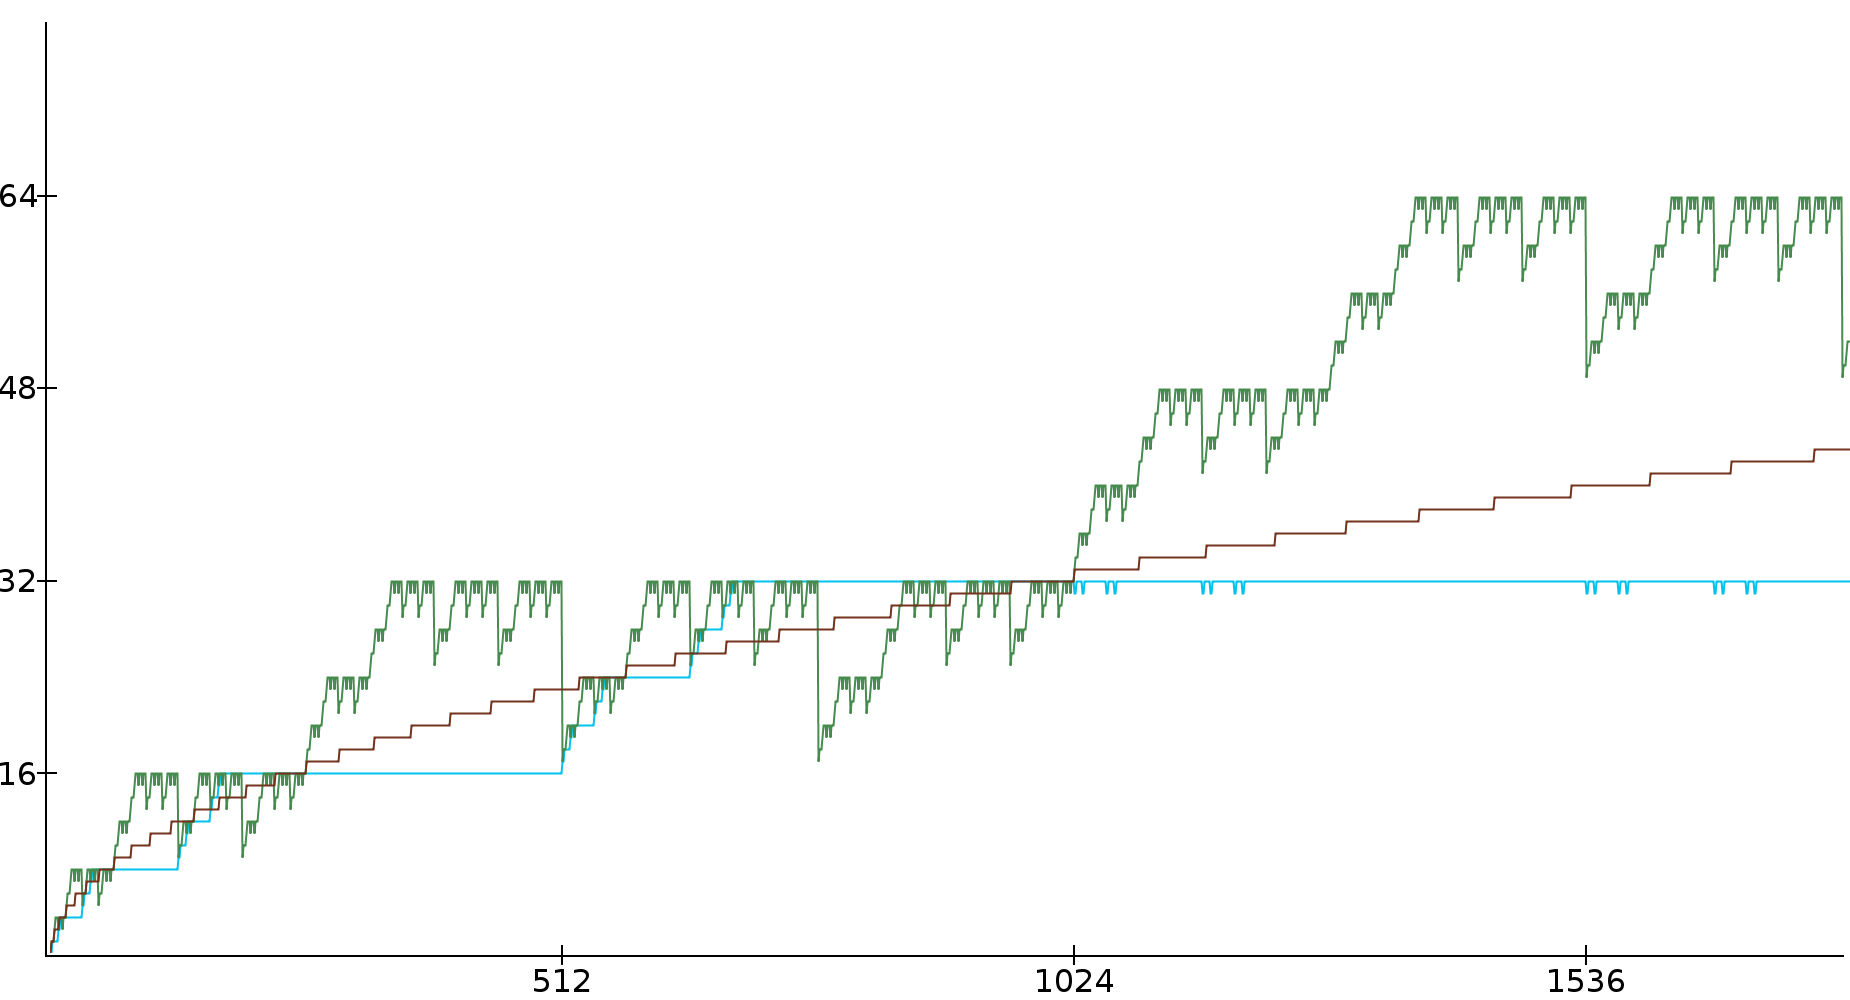
\includegraphics[width=0.75\linewidth]{figure/value12x.png} 
			\caption{Value from the simple square root approximator (green),
				the improved version (blue), and the shifting nth root 
				algorithm (red). In these graphs, they all operate on integers. 
				The shifting nth root is exact for integer square roots.}
			\label{sres1}
		\end{figure}

		\begin{figure}[H]
			\centering
			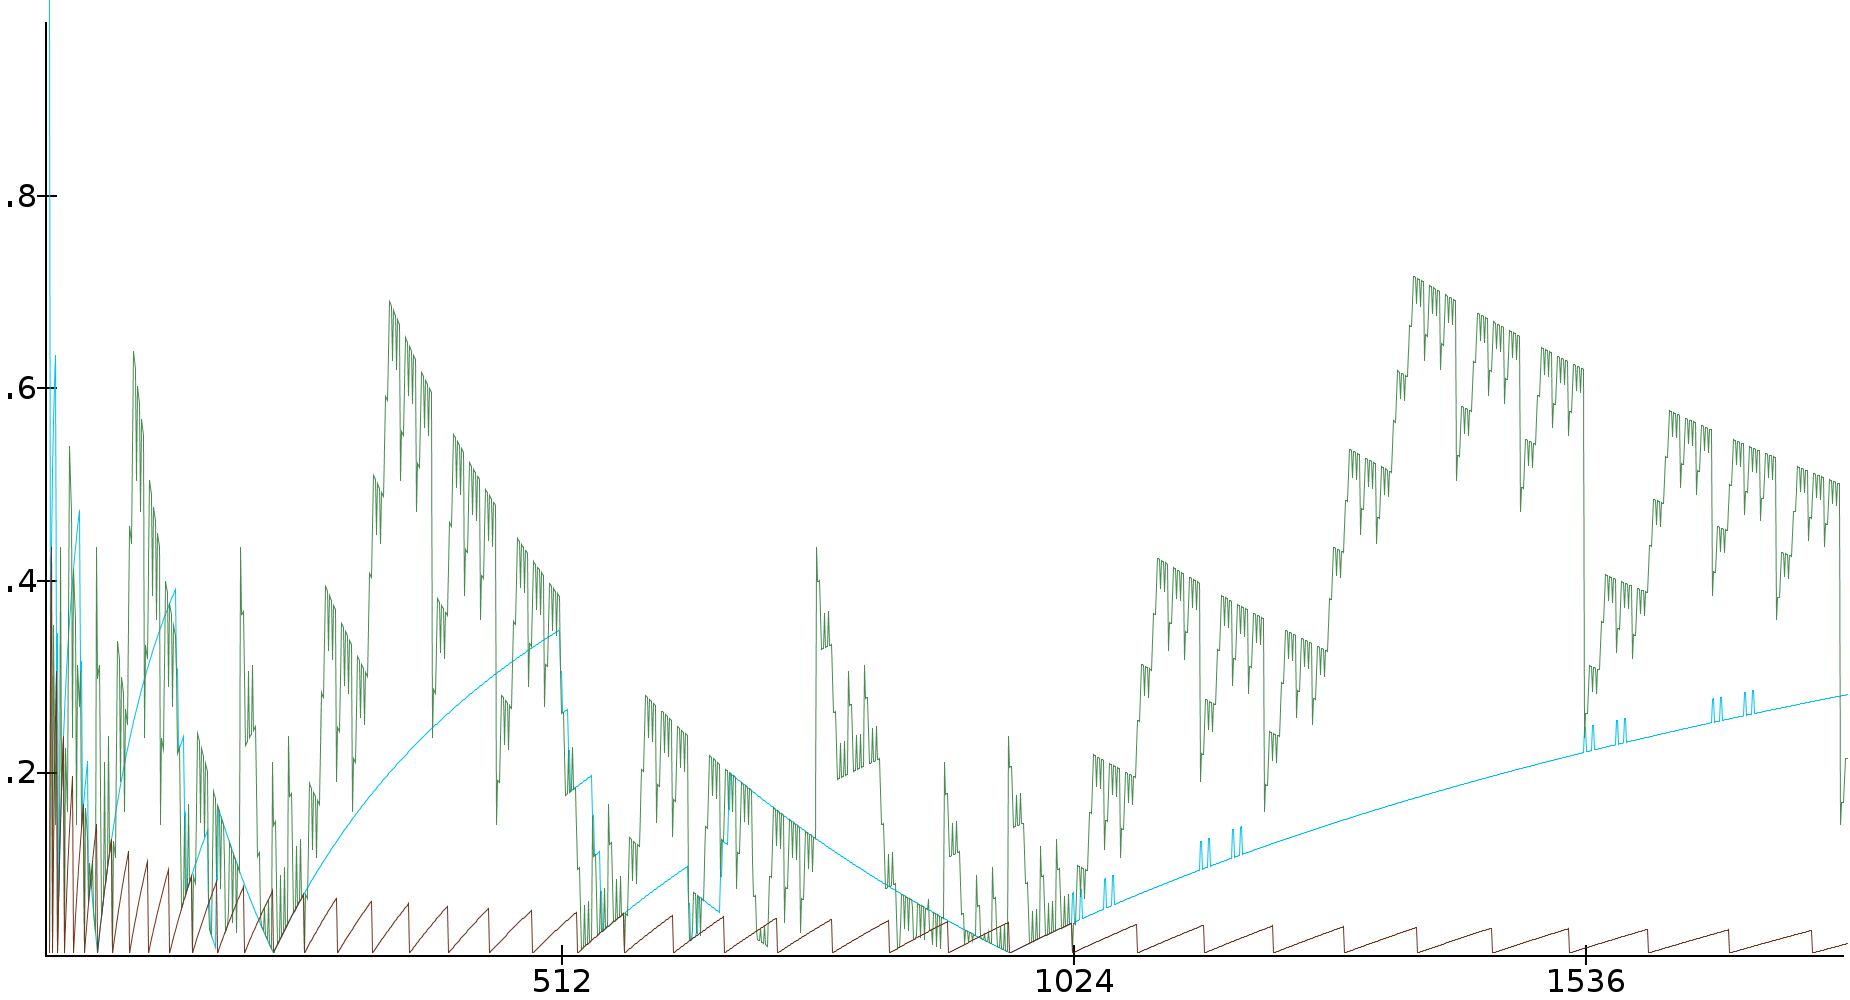
\includegraphics[width=0.75\linewidth]{figure/rel_error_480x.png} 
			\caption{Relative error for the simple square root approximator
				(green), the improved version (blue), and the shifting nth root
				algorithm (red).}
			\label{sres2}
		\end{figure}

		\begin{figure}[H]
			\centering
			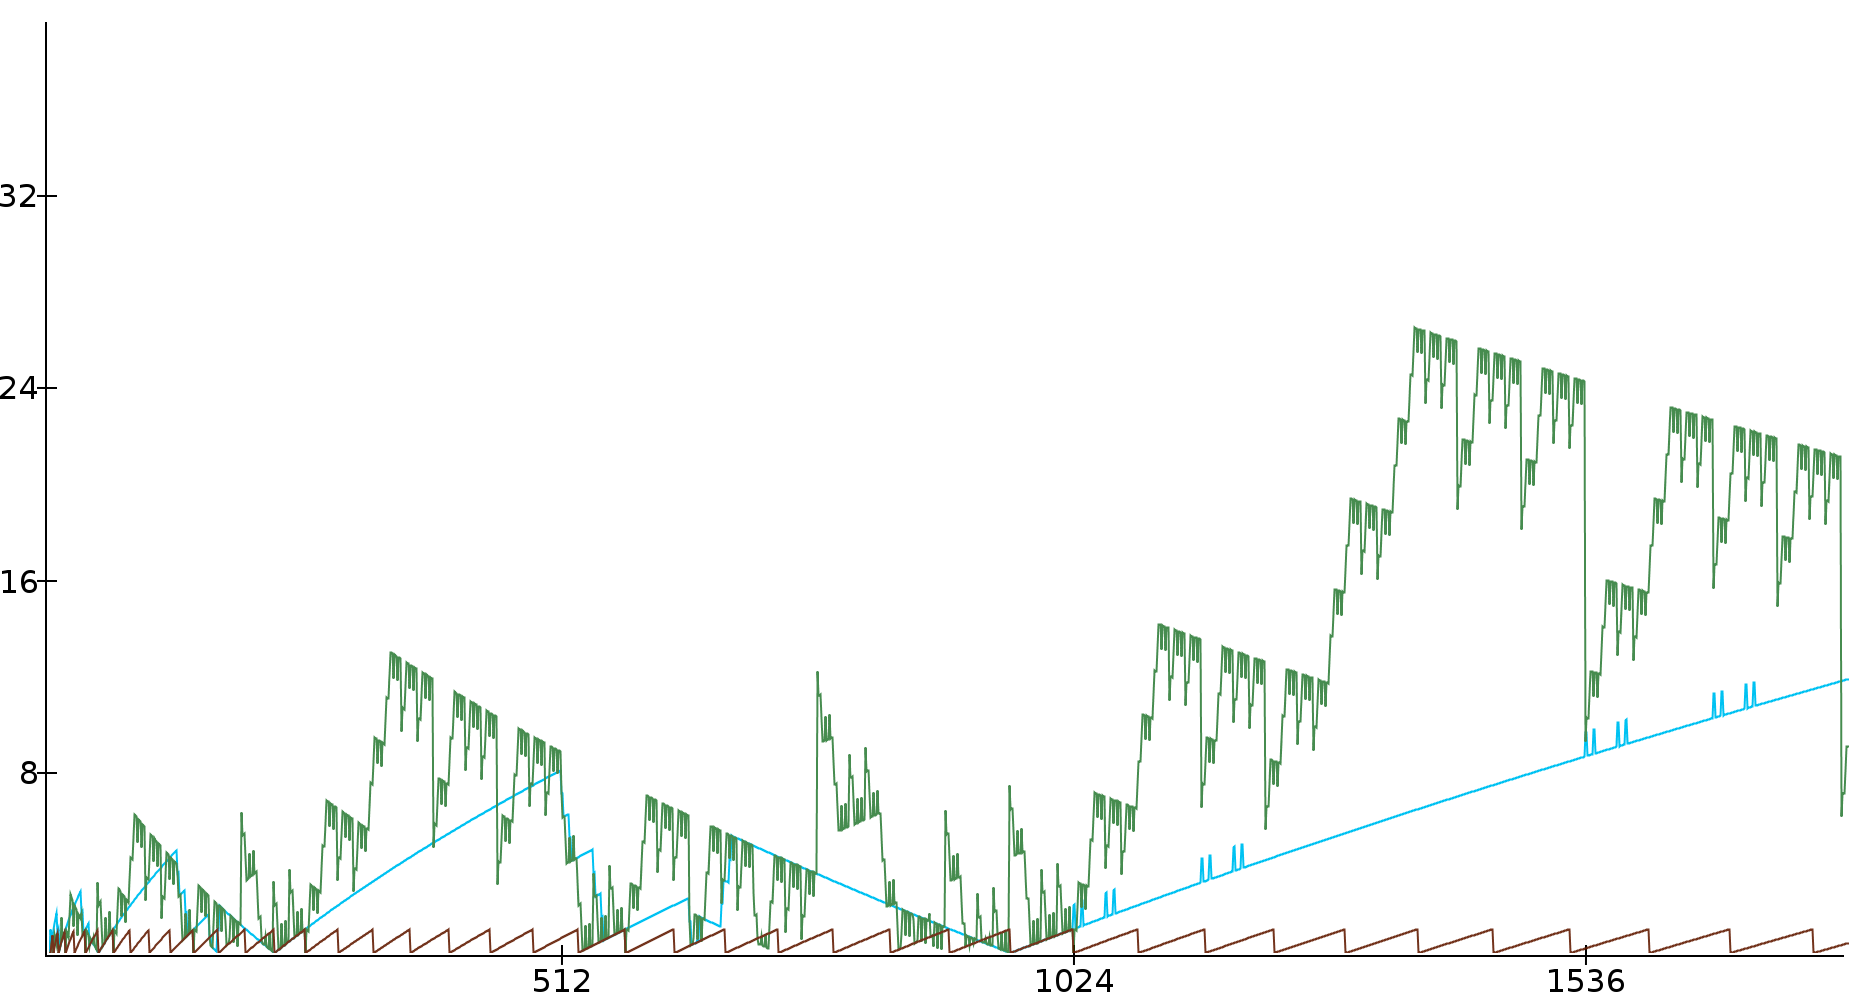
\includegraphics[width=0.75\linewidth]{figure/abs_error_24x.png} 
			\caption{Absolute error for the simple square root approximator
				(green), the improved version (blue), and the shifting nth root
				algorithm (red).}
			\label{sres3}
		\end{figure}

		\begin{figure}[H]
			\centering
			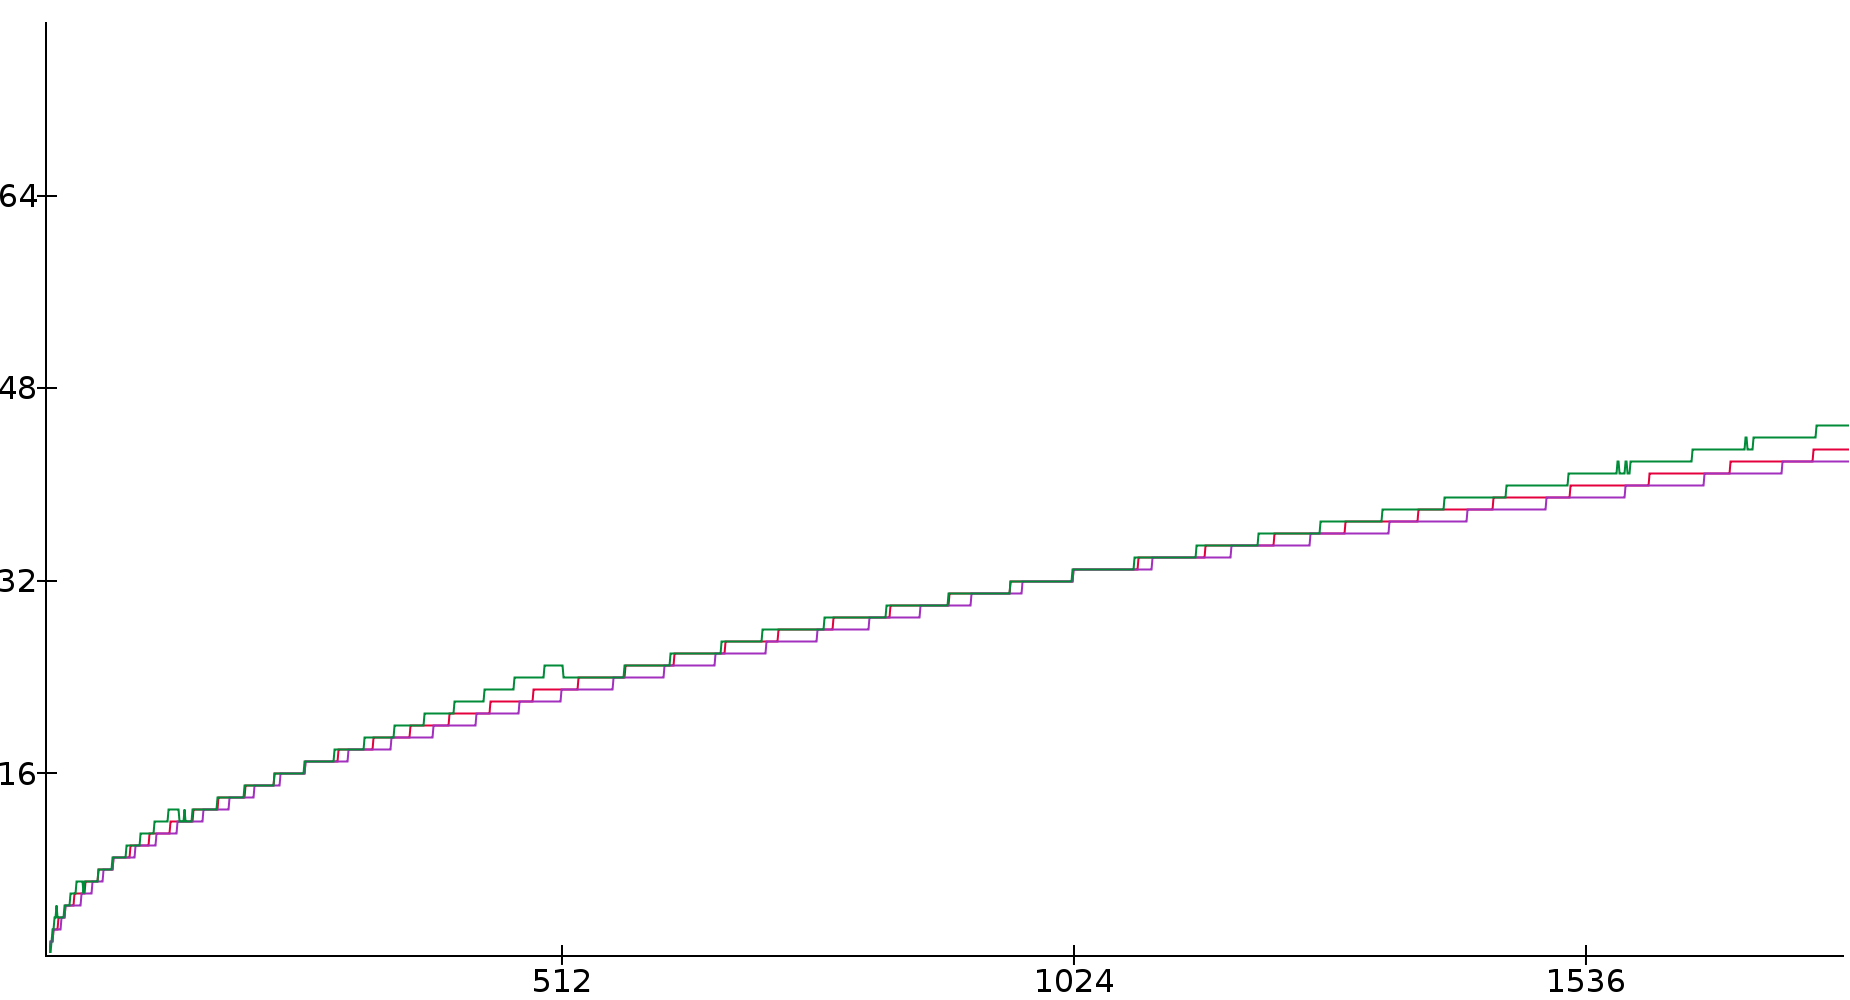
\includegraphics[width=0.75\linewidth]{figure/value_lin12x.png} 
			\caption{Value from lerp-approximator (purple), simple square root
				approximator with one step of the babylonian method (green),
				and the shifting nth root algorithm (red). In these graphs, 
				they all operate on integers. The shifting nth root is exact 
				for integer square roots.}
			\label{sres4}
		\end{figure}

		\begin{figure}[H]
			\centering
			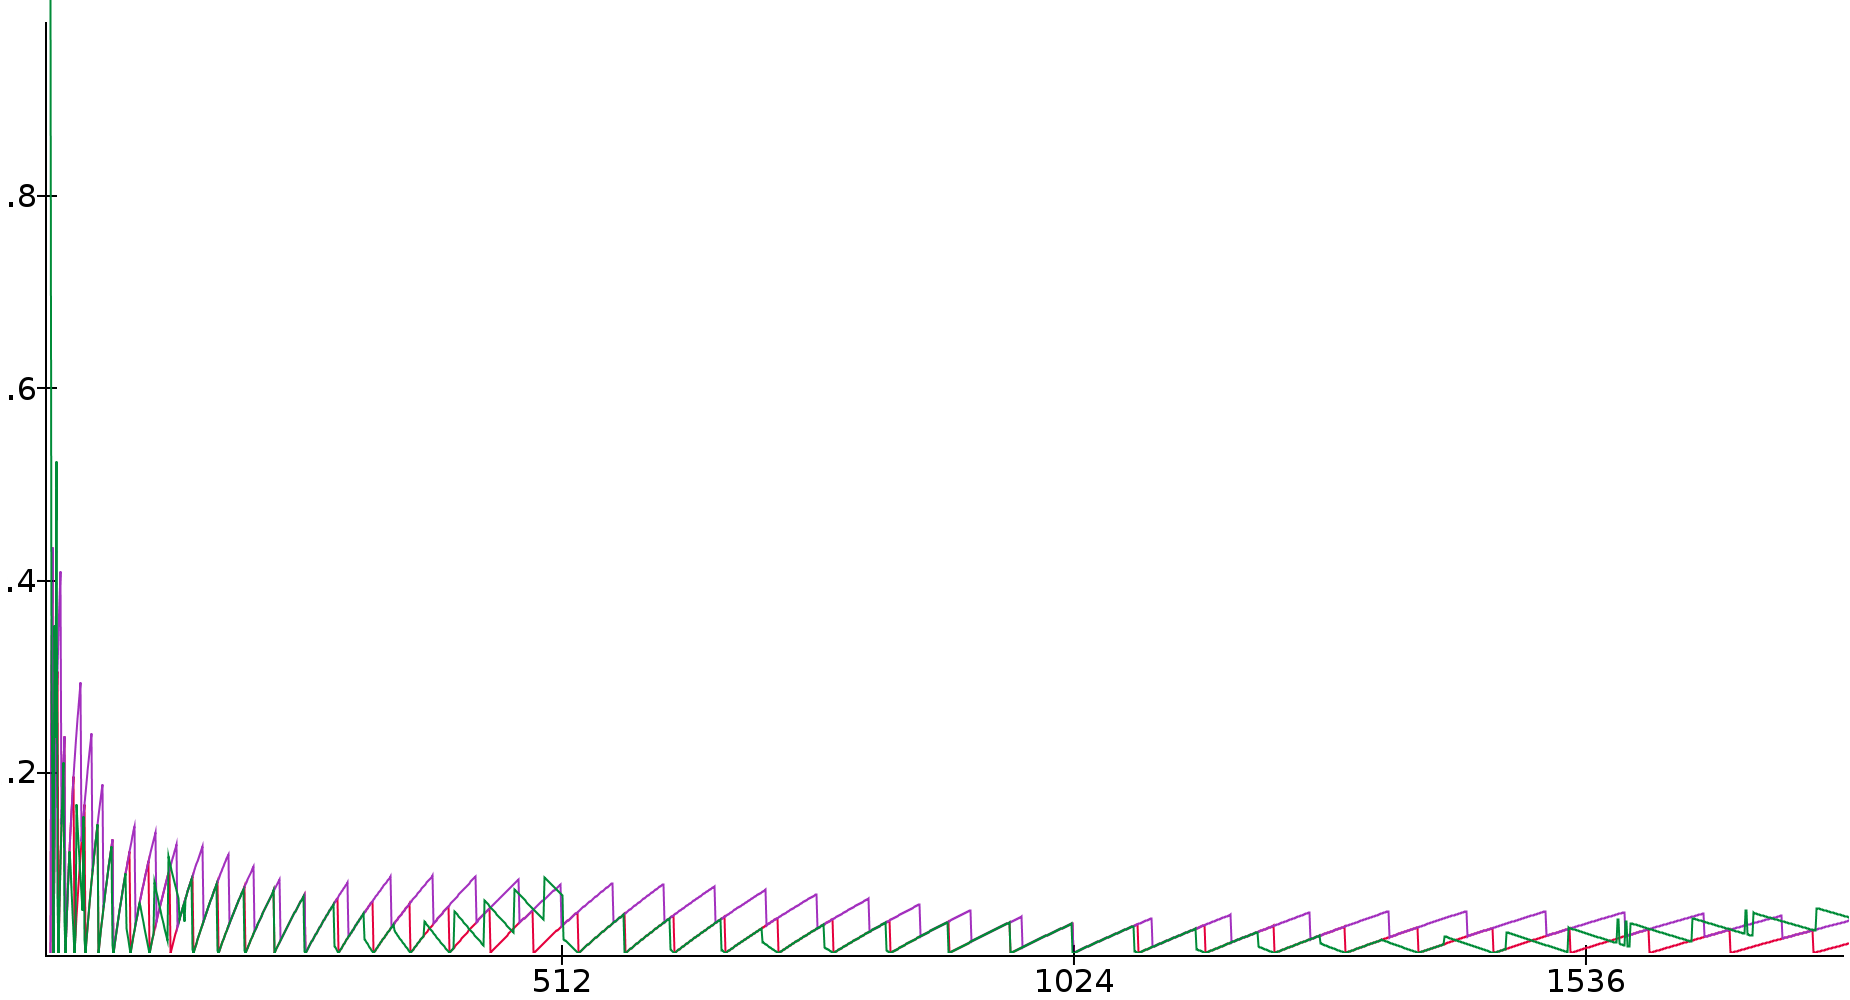
\includegraphics[width=0.75\linewidth]{figure/rel_lin960x.png} 
			\caption{Relative error for the lerp-approximator (purple), simple 
				square root approximator with one step of the babylonian method 
				(green), and the shifting nth root algorithm (red).}
			\label{sres5}
		\end{figure}

		\begin{figure}[H]
			\centering
			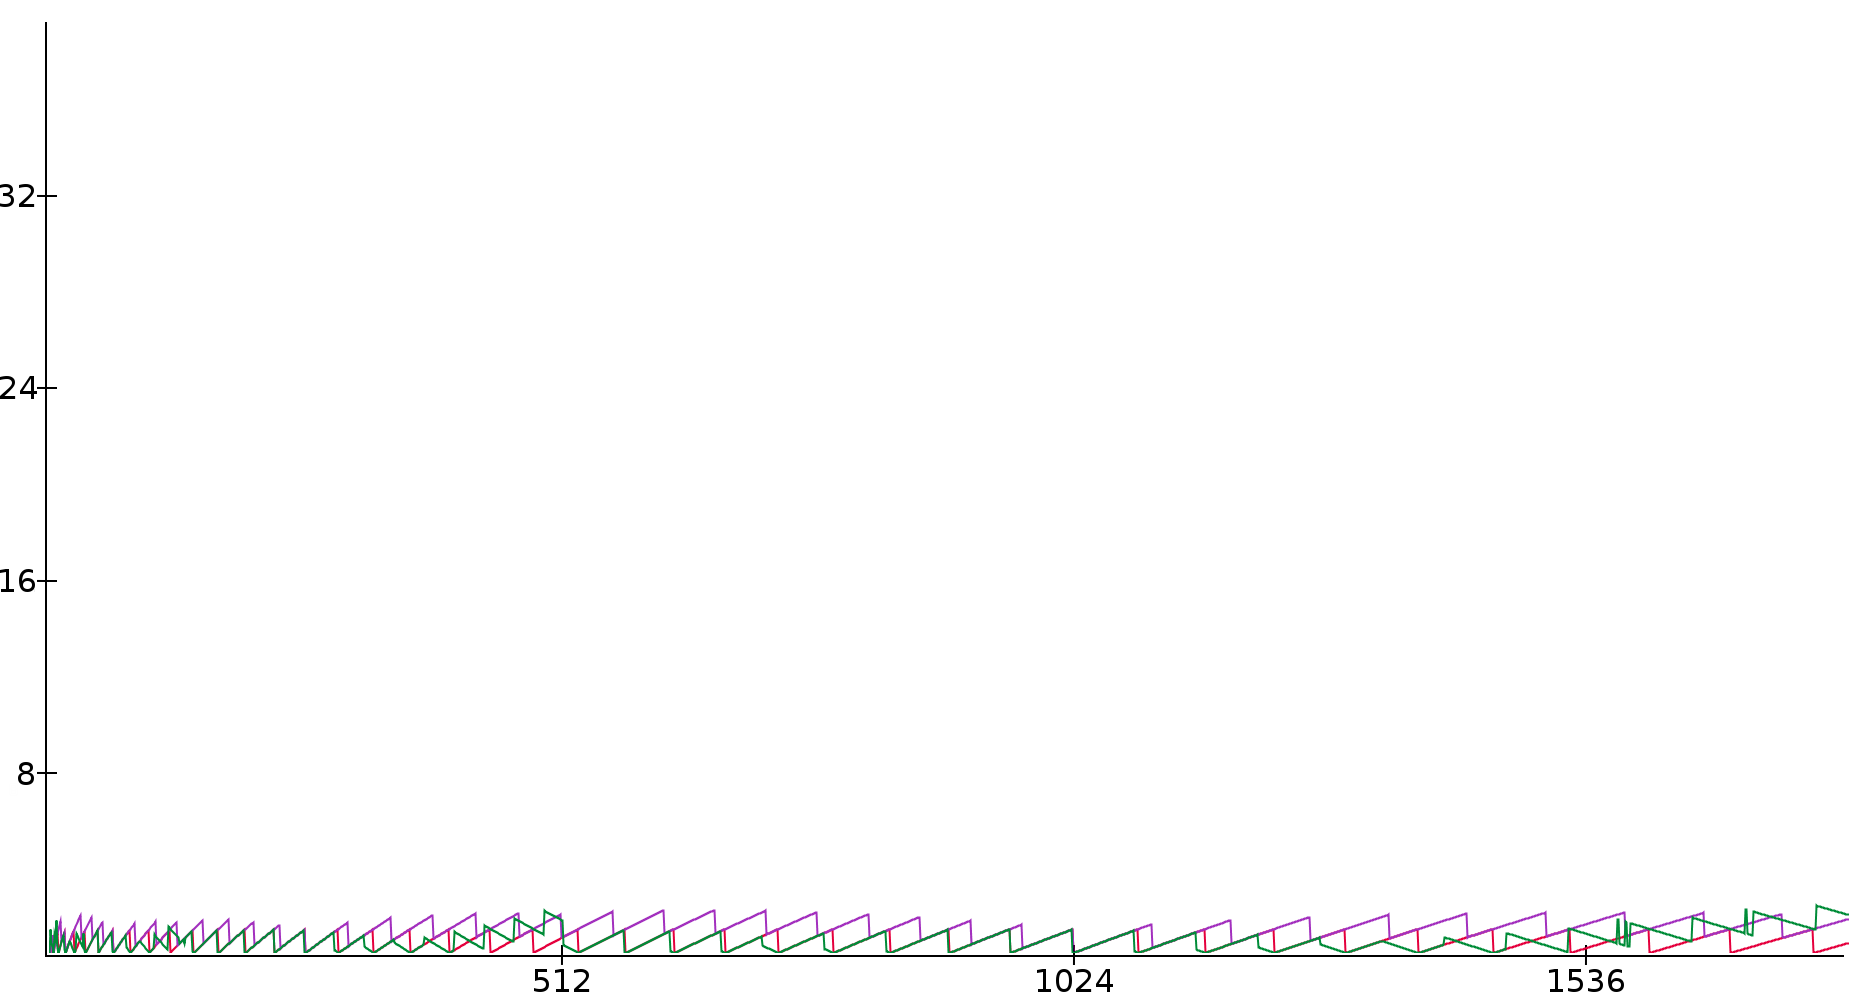
\includegraphics[width=0.75\linewidth]{figure/abs_lin24x.png} 
			\caption{Absolute error for the lerp-approximator (purple), simple 
				square root approximator with one step of the babylonian method 
				(green), and the shifting nth root algorithm (red).}
			\label{sres6}
		\end{figure}

	\section{Optimizations}
		
		During this project, a number of optimizations were discussed and
		developed. Implemented optimizations are explained below and the
		theoretical ones are presented in chapter \ref{discussion} and
		\ref{optimization}. Some of these are based on earlier work, while
		others are believed to be quite unique optimizations which have not been
		discussed for sphere tracing previously. All implemented optimizations
		that affects the algorithm were implemented in the software shader, not
		on our own GPU.

		For all tests performed, FPS (Frames Per Second) is used to measure
		performance. FPS is simply how many times the GPU is able to render 
		the scene per second. The time it takes to render the scene once is 
		equal to one divided by the FPS.

		\subsection{Orthogonal culling}
		
		Tests to see the performance of the orthogonal culling optimization
		were performed by putting an increasing number of solid-colored spheres
		in a plane in front of the camera. Because of this, the spheres are not
		obstructed by other spheres, making this the best possible scenario for
		the optimization.

		Below are test results from Orthogonal culling.

			\begin{table}
			\centering
			\begin{tabular}{lll}
				\hline
				Objects & Optimized & Unoptimized \\ 
				\hline
				1       & 600       & 350         \\ 
				5       & 430       & 180         \\			
				10      & 290       & 98          \\
				15      & 85        & 13          \\
				20      & 58        & 9           \\
				25      & 40        & 6           \\
				30      & 29        & 4           \\
				35      & 7         & 3           \\
				40      & 6         & 2           \\
				45      & 4         & 1.5         \\
				\hline
			\end{tabular}
			\caption{Frames generated per second using the GLSL shader with and
				without the orthogonal culling optimization.}
			\end{table}

			%CHARTS

		\subsection{Bounding spheres}

			Bounding spheres were implemented and tested. There was a clear
			gain in performance in some cases, but the results are very
			situational, depending on too many factors (number of objects, the
			dispersion of objects, size and place of the bounding sphere, etc.)
			to be able to review properly at this time, will be a subject of
			future work. The larger the bounding sphere, the less performance
			gain will be seen and the more objects that can fit into a bounding
			sphere the more performance gain will be seen. 


% CONCLUSION
% CREATED BY DAVID FRISK, 2016
\chapter{Conclusion}
	\section{How does sphere tracing work?}

	\section{What language is best suited to describe the GPU?}
	
	The two FHDLs, lava2000 and \clash, not being fully developed languages both produced obtuse and redundant code and in the case of \clash even unsynthezisable code (bug). In the end we decided to go with \clash and it did allow us to type less and to have a more clear overview of the GPU and its components.

	\section{Are there ways we can improve the algorithm at a theoretical level?}



	\section{How do we architect for parrallelism and multiple cores?}

	\section{How do we handle cache in a smart way?}

	\section{What mathematical functions are best implemented in hardware vs software regarding?}

% REFERENCES / BIBLIOGRAPHY
\cleardoublepage
\addcontentsline{toc}{chapter}{Bibliography}
% CREATED BY DAVID FRISK, 2016

\nocite{*}
\bibliographystyle{abbrvurl}
\bibliography{DATX02-17-12}


% APPENDICES
\cleardoublepage
\appendix
\setcounter{page}{1}
\pagenumbering{Roman}			% Capitalized roman numbering starting from I (one)

% CREATED BY DAVID FRISK, 2016
\chapter{Appendix 1}
Lorem ipsum dolor sit amet, consectetur adipisicing elit, sed do eiusmod tempor incididunt ut labore et dolore magna aliqua. Ut enim ad minim veniam, quis nostrud exercitation ullamco laboris nisi ut aliquip ex ea commodo consequat. Duis aute irure dolor in reprehenderit in voluptate velit esse cillum dolore eu fugiat nulla pariatur. Excepteur sint occaecat cupidatat non proident, sunt in culpa qui officia deserunt mollit anim id est laborum.



\end{document}
